\documentclass[12pt, a4paper]{article}

% Подключаем пакеты для расширения функциональности
\usepackage[T2A]{fontenc}   % Для кодировки шрифтов (поддержка кириллицы)
\usepackage{mathtext}
\usepackage[utf8]{inputenc} % Кодировка входного файла
\usepackage[english, russian]{babel} % Поддержка русского и английского языков
\usepackage{amsmath, amssymb} % Пакеты для математических формул (от AMS)
\usepackage{graphicx}       % Для вставки изображений
\usepackage{wrapfig}        % Для обтекания картинок текстом
\usepackage{hyperref}       % Для создания гиперссылок
\usepackage{indentfirst}    % Добавляет отступ в первом абзаце раздела
\usepackage{geometry}       % Для настройки полей
\usepackage{float}
\geometry{top=2cm, bottom=2cm, left=2.5cm, right=1.5cm} % Поля документа

\usepackage{multirow} % Для объединения ячеек по вертикали
\usepackage{array}    % Для расширенного форматирования таблиц
\usepackage{booktabs} % Для красивых горизонтальных линий (рекомендую)
\usepackage{caption}  % Для настройки подписей
\usepackage{gensymb}

\usepackage{cmap}
\usepackage[T2A]{fontenc}
\usepackage[utf8]{inputenc}

\usepackage{comment}

%---------------------------------------------------------------
\usepackage{listings} %вставка кода
\usepackage{color} % для подсветки
%\lstset{
	%language=Python, % Язык программирования
	%basicstyle=\ttfamily, % Моноширинный шрифт
	%keywordstyle=\color{blue}, % Цвет ключевых слов
	%commentstyle=\color{gray}, % Цвет комментариев
	%numbers=left, % Номера строк слева
	%frame=single % Рамка вокруг кода
%}
\definecolor{codegreen}{rgb}{0,0.6,0}
\definecolor{codegray}{rgb}{0.5,0.5,0.5}
\definecolor{codeblue}{rgb}{0,0,0.9}

\lstset{
	language=Verilog,
	basicstyle=\ttfamily\small,
	keywordstyle=\color{codeblue},
	commentstyle=\color{codegreen},
	stringstyle=\color{red},
	numbers=left,
	numberstyle=\tiny\color{codegray},
	stepnumber=1,
	numbersep=5pt,
	backgroundcolor=\color{white},
	showspaces=false,
	showstringspaces=false,
	showtabs=false,
	frame=single,
	rulecolor=\color{black},
	tabsize=2,
	captionpos=b,
	breaklines=true
}
%---------------------------------------------------------------

% Настройка метаданных PDF
\hypersetup{
	colorlinks=true,
	linkcolor=blue,
	filecolor=magenta,
	urlcolor=cyan,
	pdftitle={Пример PDF на LaTeX},
	pdfpagemode=FullScreen,
}

% Информация об авторе и заголовке
\title{\textbf{<<cnt\_en\_clr>> (счётчик с разрешением на запись и очистку)}}
\author{{Старостин Александр, Б01-401}\\{starostin.aa@phystech.edu} \\Вариант 5}
\date{\today}

% Начало документа
\begin{document}
	
	% Создание титульной страницы
	\maketitle
	\thispagestyle{empty} % Убираем номер страницы с титульного листа
	\newpage
	
	% Содержание
	\tableofcontents
	\newpage
	
	%\section{Введение}
	%\label{sec:intro}
	
	
\normalsize
	
	\section{Вступление}
	%\label{sec:work}
	
	В данном документе приведён отчёт о разработанном модуле cnt\_en\_clr (counter enable clear). Это счётчик с сигналами разрешения счёта и очистки. Код написан на языке Verilog. В качестве верификации использовались временные диаграммы. Для получения диаграм код компилировался и запускался с помощью программы <<Icarus Verilog>>. Просмотр временных диаграмм будет производиться в программе <<GTKWave>>. 
	\begin{comment}Для запуска на FPGA, код будет компилироваться и заливаться с помощью программы <<Vivado 2019.1>>. В качестве FPGA будем использовать плату <<Basys3>>.
	\end{comment}

%-----------------------------------------------------------------------
	\section{Документация разрабатываемого модуля}
	
	В данном разделе приведена документация к разрабатываемому модулю. Документация включает в себя следующие разделы: функциональное описание, структурная схема, параметры, порты, тактирование и сброс, тестирование.

%-----------------------------------------------------------------------
	\subsection{Функциональное описание}
	
	Опишем функционал разрабатываемого модуля. \\
	
	Модуль <<cnt\_en\_clr>> -- это счётчик, который меняет своё значение по положительному фронту такового сигнала (увеличивает значение на 1, при выставленном сигнале разрешения записи; обнуляется при выставленном сигнале очистки (очистка приоритетнее, чем запись); в противном случае - сохраняет своё значение) и по отрицательному фронту сигнала сброса (сигнал сброса приоритетнее, чем тактовый сигнал).   \\
	
	Размер счётчика может варьироваться с помощью параметра.\\
	
	Кроме самого значения счётчика хранится информация о переполнении счёта. Для этого имеется сигнал переполнения. К примеру, если счётчик 4-х битный и до положительного фронта тактового сигнала имеет значение 1111 в двоичной СИ (сигнал переполнения выставлен в 0), то после положительного фронта (при разрешении на запись и запрете на очистку) счётчик станет хранит значение 0000, а сигнал переполнения -- 1. Повторное переполнение не обрабатывается, т.е. при повторном переполнении счётчика сигнал переполнения станет равным 0. Обработка повторного переполнения не предусмотрена, тк она усложнит логику разрабатываемого модуля и увеличит его критический путь (зависит от реализации обработки). Так что будем считать, что двойное переполнение не является ожидаемым поведением и что при первом переполнении последует его программная обработка со стороны пользователя (например, через программу на ассемблере). \\
	
	При очистке и сбросе обнуляются значения и счётчика, и сигнала переполнения. В таком случае они принимают значение: 0. \\
	
	Счётчик реагирует только на положительный фронт тактового сигнала или на отрицательный фронт сигнала сброса. Логика модуля устроена так, что она имеет свои приоритеты, и обработка этих событий осуществляется по приоритетам в 3 этапа. Рассмотрим прохождение по этим этапам:
	
	1. Если произошло одно из этих событий, то счётчик проверяет значение сигнала сброса. Если оно в данный момент выставлено в 0 (вне зависимости от 'триггерного' события), то значение счетчика и сигнала переполнения выставляются в 0. На этом работа счётчика заканчивается до следующего события. 
	
	2. Если обработка события дошла до этого этапа, то сигнал сброса равен 1. А значит, что произошёл именно положительный фронт тактового сигнала. На этом проверяется значение сигнала очистки. Если оно выставлено в 1, то значения счётчика и сигнала переполнения обнуляются. На этом обработка события заканчивается. 
	
	3. На этом этапе происходит стандартное изменение значения счётчика. Если сигнал разрешения счёта выставлен в 1, то значение счётчика увеличивается на 1 (с возможностью переполнения). Иначе -- значение счётчика сохраняется. \\

	Заметим, что и сигнал сброса, и сигнал очистки блокируют продолжение увеличения счётчика (вне зависимости от сигнала разрешения счёта). Но они отличаются тем, что сигнал сброса (при отрицательном фронте) мгновенно обнуляет значение счётчика и сигнала переполнения (асинхронно с тактовым сигналом), а сигнал очистки, если он выставлен в 1 -- только при положительном фронте тактового  сигнала (синхронно с тактовым сигналом).
		
%-----------------------------------------------------------------------	
	\subsection{Структурная схема}
	
	Ниже представлена структурная схема разрабатываемого счётчика. Тонкими стрелками обозначаются шины размером 1 бит. Толстые с одной чертой -- N бит. Толстые с двумя черточками -- N+1 бит. N - размер счётчика в битах. \\
	
	Порты, на конце которых присутствуют <<i>> или <<o>>, будут описаны позже. Порт 
	<<cnt\_internal>>
	является внутренним и используется для хранения значения счетчика и сигнала переполнения. Его значение в данный момент времени определяют входные порты. Далее этот порт разбивается на выходные порты.
	
	\begin{figure}[H]
		\centering
		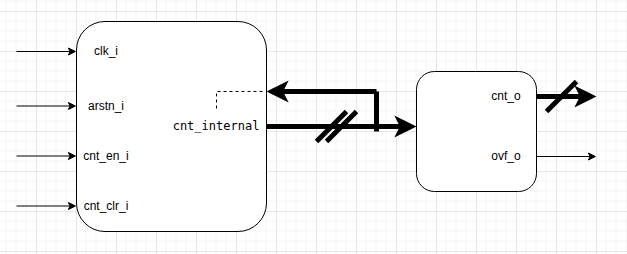
\includegraphics[width=0.9\linewidth]{./pictures/block_diagram.png}
		\caption{Структурная схема модуля <<cnt\_en\_clr>>}
		\label{fig:block_diagram}
	\end{figure}
	
%-----------------------------------------------------------------------
	\subsection{Параметры}
	
	Модуль имеет параметр CNT\_WIDTH для указания размера счетчика в битах. Допустимые значения параметра: положительные целые числа (CNT\_WIDTH -- целое; CNT\_WIDTH >= 1).
	
%-----------------------------------------------------------------------
	\subsection{Порты}
	
	Модуль имеет следующие порты:
	
	\begin{table}[H]
		\centering
		\begin{tabular}{|p{2.5cm}|c|c|p{5cm}|}
			\hline
			\textbf{Название} & \textbf{Ширина} & \textbf{Направление} & \textbf{Описание} \\
			\hline
			clk\_i & 1 & Input & Тактовый сигнал \\
			\hline
			arstn\_i & 1 & Input & Сигнал сброса \\
			\hline
			cnt\_en\_i & 1 & Input & Сигнал разрешения счёта \\
			\hline
			cnt\_clr\_i & 1 & Input & Сигнал очистки \\
			\hline
			cnt\_o & CNT\_WIDTH & Output & Значение счётчика \\
			\hline
			ovf\_o & 1 & Output & Сигнал переполнения \\
			\hline
		\end{tabular}
		
		\caption{Описание портов счетчика}
		\label{tab:counter_ports}
	\end{table}
	
	О <<clk\_i>> и <<arstn\_i>> будет рассказано ниже.
	
	<<cnt\_en\_i>> -- разрешает или запрещает продолжать увеличение счётчика на 1.
	
	<<cnt\_clr\_i>> -- разрешает или запрещает очистку значений счётчика и сигнала переполнения.
	
%-----------------------------------------------------------------------
	\subsection{Тактирование и сброс}
	
	Тактирование осуществляется сигналом <<clk\_i>> по положительному фронту. \\
	
	Сброс осуществляется сигналом <<arstn\_i>> по отрицательному фронту. Т.е., когда значение <<arstn\_i>> меняется с 1 на 0, мгновенно обнуляются значения счетчика и сигнала переполнения и, пока значение <<arstn\_i>> = 0, блокируется вся работа счётчика, а его значение остаётся равным 0 (см. описание приоритетной по этапам реакции счётчика на тактирование и сброс).
	
%-----------------------------------------------------------------------
	\subsection{Тестирование}
	
	Тестирование будем проводить с помощью двух сценариев: testbench всего функционала счётчика, кроме переполнения и testbench только с переполнением. Более подробно об этих сценариях будет рассказано ниже.
	
%-----------------------------------------------------------------------
\section{Скачивание и запуск кода}

Прежде чем мы рассмотрим реализацию модуля на Verilog следует заметить, что для более удобного просмотра кода его можно смотреть на моём \href{https://github.com/Alexandr26Starostin/counter_enable_clear}{\textbf{репозитории}} (код выложен после дедлайна!!!). \\

Далее идёт описание для скачивания и запуска кода на Linux Ubuntu. Сначала устанавливаем <<Icarus Verilog>> и <<GTKWave>>:
\begin{verbatim}
	sudo apt update
	sudo apt install iverilog
	sudo apt install gtkwave
\end{verbatim}

После клонируем репозиторий в свою директорию:
\begin{verbatim}
	git clone https://github.com/Alexandr26Starostin/counter_enable_clear
\end{verbatim}

Далее мы будем указывать команды, чтобы компилировать и тестировать с помощью диаграмм наш модуль. 
	
%-----------------------------------------------------------------------
	\section{Файл с имплементацией разработанного модуля}

Ниже представлена реализация модуля <<cnt\_en\_clr>> на языке Verilog в соответствии с требованиями: \\
	
\begin{lstlisting}[caption={Содержимое файла ./hdl/counter.v}, label={lst:example}]
//file ./hdl/counter.v
//module cnt_en_clr - counter_enable_clear 
//---------------------------------------------

//`define FPGA //-- if we use FPGA, we need in button's delay (because button is the clk)
//------------------------------------
`ifdef FPGA
`timescale 1ns / 1ps    //for button's delay
`endif
//------------------------------------

module cnt_en_clr #(
	parameter CNT_WIDTH = 8   //size of counter
)(
	input                    clk_i,
	input                    arstn_i, //reset -  synchronous with clk
                                    //      - asynchronous with clk (we use it!)
	input                    cnt_en_i,
	input                    cnt_clr_i,

	output [CNT_WIDTH -1 :0] cnt_o,
	output                   ovf_o 
);

reg [CNT_WIDTH :0] cnt_internal;
//reg                clr_execute;

always @(posedge clk_i or negedge arstn_i) begin
	if (! arstn_i) begin       //reset  ->  //ovf_o == '0 | cnt_o  == '0                              (immediately after negedge arstn_i)  
		cnt_internal <= {CNT_WIDTH + 1{1'b0}};   //cnt_internal <= '0;
	end 

	else if (cnt_clr_i) begin  //clear  ->  //ovf_o == '0 | cnt_o  == '0  	                        (immediately after posedge clk_i)  
		cnt_internal <= {CNT_WIDTH + 1{1'b0}};   //cnt_internal <= '0;
	end

	else begin
		cnt_internal <= cnt_en_i ? cnt_internal + 1 : cnt_internal; 
	end

	//------------------------------------
	`ifdef FPGA 
	#1000;
	`endif
	//------------------------------------
end

assign {ovf_o, cnt_o} = cnt_internal;

endmodule

\end{lstlisting}

%-----------------------------------------------------------------------
	\section{Файлы с testbench для разработанного модуля}

Теперь предложим два файлы с testbench: один -- для всего функционала модуля, другой только для переполнения. О сценариях тестирования будет сказано во время анализа временных диаграмм.

%---------------------------------------------------------------------------------------------------------------------------------------------------------------------------------

	\subsection{Файл с testbench для всего функционала модуля, кроме сигнала переполнения} 

\begin{lstlisting}[caption={Содержимое файла ./tb/tb.v}, label={lst:example}]
	
//file ./tb/tb.v
	
`timescale 1ns/1ps
	
//----------------------------
`define GUI_ENABLED
//----------------------------
	
module cnt_en_clr_tb ();
	
//------------------------------------------------
	
localparam CNT_WIDTH = 8;
	
reg                   clk_i;
reg                   arstn_i;
reg                   cnt_en_i;
reg                   cnt_clr_i;
wire [CNT_WIDTH-1 :0] cnt_o;
wire                  ovf_o;
	
cnt_en_clr #(
	.CNT_WIDTH  (CNT_WIDTH)
) cnt_en_clr_inst_tb (
	.clk_i     (clk_i),
	.arstn_i   (arstn_i),
	
	.cnt_en_i  (cnt_en_i),
	.cnt_clr_i (cnt_clr_i),
	
	.cnt_o     (cnt_o),
	.ovf_o     (ovf_o)
);
	
//------------------------------------------------
//graphic dump
	
`ifdef GUI_ENABLED 
initial begin
	$dumpvars;
	
	clk_i      = 1'b0;     
	arstn_i    = 1'b1;      
	cnt_en_i   = 1'b0;
	cnt_clr_i  = 1'b0;
	#4;
	
	clk_i      = 1'b0;
	arstn_i    = 1'b0;
	cnt_en_i   = 1'b0;
	cnt_clr_i  = 1'b0;
	#6;                       //10
	
	clk_i      = 1'b1;
	arstn_i    = 1'b0;
	cnt_en_i   = 1'b0;
	cnt_clr_i  = 1'b0;        //20
	#10
	
	clk_i      = 1'b0;
	arstn_i    = 1'b0;
	cnt_en_i   = 1'b0;
	cnt_clr_i  = 1'b0;
	#5
	
	clk_i      = 1'b0;
	arstn_i    = 1'b0;
	cnt_en_i   = 1'b1;
	cnt_clr_i  = 1'b0;
	#5                         //30
	
	clk_i      = 1'b1;
	arstn_i    = 1'b0;
	cnt_en_i   = 1'b1;
	cnt_clr_i  = 1'b0;
	#4
	
	clk_i      = 1'b1;
	arstn_i    = 1'b1;
	cnt_en_i   = 1'b1;
	cnt_clr_i  = 1'b0;
	#6                        //40
	
	clk_i      = 1'b0;
	arstn_i    = 1'b1;
	cnt_en_i   = 1'b1;
	cnt_clr_i  = 1'b0;
	#10                       //50
	
	clk_i      = 1'b1;
	arstn_i    = 1'b1;
	cnt_en_i   = 1'b1;
	cnt_clr_i  = 1'b0;
	#10                      //60
	
	clk_i      = 1'b0;
	arstn_i    = 1'b1;
	cnt_en_i   = 1'b1;
	cnt_clr_i  = 1'b0;
	#10                      //70
	
	clk_i      = 1'b1;
	arstn_i    = 1'b1;
	cnt_en_i   = 1'b1;
	cnt_clr_i  = 1'b0;
	#5
	
	clk_i      = 1'b1;
	arstn_i    = 1'b1;
	cnt_en_i   = 1'b0;
	cnt_clr_i  = 1'b0;
	#5                      //80
	
	clk_i      = 1'b0;
	arstn_i    = 1'b1;
	cnt_en_i   = 1'b0;
	cnt_clr_i  = 1'b0;
	#10                      //90
	
	clk_i      = 1'b1;
	arstn_i    = 1'b1;
	cnt_en_i   = 1'b0;
	cnt_clr_i  = 1'b0;
	#10                      //100
	
	clk_i      = 1'b0;
	arstn_i    = 1'b1;
	cnt_en_i   = 1'b0;
	cnt_clr_i  = 1'b0;
	#3
	
	clk_i      = 1'b0;
	arstn_i    = 1'b1;
	cnt_en_i   = 1'b1;
	cnt_clr_i  = 1'b0;
	#7                      //110
	
	clk_i      = 1'b1;
	arstn_i    = 1'b1;
	cnt_en_i   = 1'b1;
	cnt_clr_i  = 1'b0;
	#10                      //120
	
	clk_i      = 1'b0;
	arstn_i    = 1'b1;
	cnt_en_i   = 1'b1;
	cnt_clr_i  = 1'b0;
	#6
	
	clk_i      = 1'b0;
	arstn_i    = 1'b1;
	cnt_en_i   = 1'b1;
	cnt_clr_i  = 1'b1;
	#4                       //130
	
	clk_i      = 1'b1;
	arstn_i    = 1'b1;
	cnt_en_i   = 1'b1;
	cnt_clr_i  = 1'b1;
	#10                    //140
	
	clk_i      = 1'b0;
	arstn_i    = 1'b1;
	cnt_en_i   = 1'b1;
	cnt_clr_i  = 1'b1;
	#7
	
	clk_i      = 1'b0;
	arstn_i    = 1'b1;
	cnt_en_i   = 1'b1;
	cnt_clr_i  = 1'b0;
	#3                      //150
	
	clk_i      = 1'b1;
	arstn_i    = 1'b1;
	cnt_en_i   = 1'b1;
	cnt_clr_i  = 1'b0;
	#10                     //160
	
	clk_i      = 1'b0;
	arstn_i    = 1'b1;
	cnt_en_i   = 1'b1;
	cnt_clr_i  = 1'b0;
	#10                     //170
	
	clk_i      = 1'b1;
	arstn_i    = 1'b1;
	cnt_en_i   = 1'b1;
	cnt_clr_i  = 1'b0;
	#10                     //180
	
	//--------------------------------------------------------
	
	clk_i      = 1'b0;
	arstn_i    = 1'b1;
	cnt_en_i   = 1'b1;
	cnt_clr_i  = 1'b0;
	#10                     //190
	
	clk_i      = 1'b1;
	arstn_i    = 1'b1;
	cnt_en_i   = 1'b1;
	cnt_clr_i  = 1'b0;
	#10                     //200
	
	//--------------------------------------------------------
	
	clk_i      = 1'b0;
	arstn_i    = 1'b1;
	cnt_en_i   = 1'b1;
	cnt_clr_i  = 1'b0;
	#4                     
	
	clk_i      = 1'b0;
	arstn_i    = 1'b1;
	cnt_en_i   = 1'b0;
	cnt_clr_i  = 1'b0;
	#2
	
	clk_i      = 1'b0;
	arstn_i    = 1'b1;
	cnt_en_i   = 1'b0;
	cnt_clr_i  = 1'b1;
	#3                     //210      
	
	clk_i      = 1'b1;
	arstn_i    = 1'b1;
	cnt_en_i   = 1'b0;
	cnt_clr_i  = 1'b1;
	#10                     //220
	
	clk_i      = 1'b0;
	arstn_i    = 1'b1;
	cnt_en_i   = 1'b0;
	cnt_clr_i  = 1'b1;
	#10                     //230
	
	//------------------------------------------------------------------
	// $display();
	// $display("------------------------------------------------------------");
	// $display ("PASS: 'multibit_adder' test PASSED!");
	// $display("------------------------------------------------------------");
	// $display();
	
	$finish;
end
`endif
	
//----------------------------------------------
//generating of tests  
`ifndef GUI_ENABLED
`endif
	
//-----------------------------------------------------
//reaction --  automatic verification
	
endmodule
		
\end{lstlisting}

%---------------------------------------------------------------------------------------------------------------------------------------------------------------------------------
	
	\subsection{Файл с testbench для переполнения} 

\begin{lstlisting}[caption={Содержимое файла ./tb/tb\_overflow.v}, label={lst:example}]
	
//file ./tb/tb_overflow.v

`timescale 1ns/1ps

//----------------------------
`define GUI_ENABLED
//----------------------------

module cnt_en_clr_tb ();

//--------------------------------------------------

localparam CNT_WIDTH = 2;  //max_cnt_value = 2**2 - 1 = 3

reg                   clk_i;
reg                   arstn_i;
reg                   cnt_en_i;
reg                   cnt_clr_i;
wire [CNT_WIDTH-1 :0] cnt_o;
wire                  ovf_o;

cnt_en_clr #(
	.CNT_WIDTH  (CNT_WIDTH)
) cnt_en_clr_inst_tb (
	.clk_i     (clk_i),
	.arstn_i   (arstn_i),

	.cnt_en_i  (cnt_en_i),
	.cnt_clr_i (cnt_clr_i),

	.cnt_o     (cnt_o),
	.ovf_o     (ovf_o)
);

//-----------------------------------------------
//graphic dump

`ifdef GUI_ENABLED 
initial begin
	$dumpvars;

	//--------------------------------------------------------

	clk_i      = 1'b1;
	arstn_i    = 1'b1;
	cnt_en_i   = 1'b0;
	cnt_clr_i  = 1'b0;
	#3                     

	clk_i      = 1'b1;
	arstn_i    = 1'b0;
	cnt_en_i   = 1'b0;
	cnt_clr_i  = 1'b0;
	#3                     
	
	clk_i      = 1'b1;
	arstn_i    = 1'b1;
	cnt_en_i   = 1'b1;
	cnt_clr_i  = 1'b0;
	#4                     //10
	
	//=0_00
	//--------------------------------------------------------
	
	clk_i      = 1'b0;
	arstn_i    = 1'b1;
	cnt_en_i   = 1'b1;
	cnt_clr_i  = 1'b0;
	#10                     //20
	
	clk_i      = 1'b1;
	arstn_i    = 1'b1;
	cnt_en_i   = 1'b1;
	cnt_clr_i  = 1'b0;
	#10                     //30
	
	//=0_01
	//--------------------------------------------------------
	
	//--------------------------------------------------------
	
	clk_i      = 1'b0;
	arstn_i    = 1'b1;
	cnt_en_i   = 1'b1;
	cnt_clr_i  = 1'b0;
	#10                     //40
	
	clk_i      = 1'b1;
	arstn_i    = 1'b1;
	cnt_en_i   = 1'b1;
	cnt_clr_i  = 1'b0;
	#10                     //50
	
	//=0_10
	//--------------------------------------------------------
	
	
	//--------------------------------------------------------
	
	clk_i      = 1'b0;
	arstn_i    = 1'b1;
	cnt_en_i   = 1'b1;
	cnt_clr_i  = 1'b0;
	#10                     //60
	
	clk_i      = 1'b1;
	arstn_i    = 1'b1;
	cnt_en_i   = 1'b1;
	cnt_clr_i  = 1'b0;
	#10                     //70
	
	//=0_11
	//--------------------------------------------------------
	
	//--------------------------------------------------------
	
	clk_i      = 1'b0;
	arstn_i    = 1'b1;
	cnt_en_i   = 1'b1;
	cnt_clr_i  = 1'b0;
	#10                     //80
	
	clk_i      = 1'b1;
	arstn_i    = 1'b1;
	cnt_en_i   = 1'b1;
	cnt_clr_i  = 1'b0;
	#10                     //90
	
	//=1_00
	//--------------------------------------------------------
	
	//--------------------------------------------------------
	
	clk_i      = 1'b0;
	arstn_i    = 1'b1;
	cnt_en_i   = 1'b1;
	cnt_clr_i  = 1'b0;
	#10                     //100
	
	clk_i      = 1'b1;
	arstn_i    = 1'b1;
	cnt_en_i   = 1'b1;
	cnt_clr_i  = 1'b0;
	#10                     //110
	
	//=1_01
	//--------------------------------------------------------
	
	//--------------------------------------------------------
	
	clk_i      = 1'b0;
	arstn_i    = 1'b1;
	cnt_en_i   = 1'b1;
	cnt_clr_i  = 1'b0;
	#10                     //120
	
	clk_i      = 1'b1;
	arstn_i    = 1'b1;
	cnt_en_i   = 1'b1;
	cnt_clr_i  = 1'b0;
	#10                     //130
	
	//=1_10
	//--------------------------------------------------------
	
	//--------------------------------------------------------
	
	clk_i      = 1'b0;
	arstn_i    = 1'b1;
	cnt_en_i   = 1'b1;
	cnt_clr_i  = 1'b0;
	#10                     //140
	
	clk_i      = 1'b1;
	arstn_i    = 1'b1;
	cnt_en_i   = 1'b1;
	cnt_clr_i  = 1'b0;
	#10                     //150
	
	//=1_11
	//--------------------------------------------------------
	
	//--------------------------------------------------------
	
	clk_i      = 1'b0;
	arstn_i    = 1'b1;
	cnt_en_i   = 1'b1;
	cnt_clr_i  = 1'b0;
	#10                     //160
	
	clk_i      = 1'b1;
	arstn_i    = 1'b1;
	cnt_en_i   = 1'b1;
	cnt_clr_i  = 1'b0;
	#10                     //170
	
	//=0_00
	//--------------------------------------------------------
	
	//--------------------------------------------------------
	
	clk_i      = 1'b0;
	arstn_i    = 1'b1;
	cnt_en_i   = 1'b1;
	cnt_clr_i  = 1'b0;
	#10                     //180
	
	clk_i      = 1'b1;
	arstn_i    = 1'b1;
	cnt_en_i   = 1'b1;
	cnt_clr_i  = 1'b0;
	#10                     //190
	
	//=0_01
	//--------------------------------------------------------
	
	$finish;
end
`endif

endmodule

\end{lstlisting}
	
	
%-----------------------------------------------------------------------
	\section{Временные диаграммы}
	
	Все диаграммы можно посмотреть в директории <<./pictures>>.
	
%-----------------------------------------------------------------------
	\subsection{testbench для всего функционала модуля, кроме сигнала переполнения}
	
	Чтобы увидеть временную диаграмму <<dump\_1.png>> или <<dump\_1.jpg>>, выполняем следующие команды:
	
	\begin{verbatim}
	iverilog ./hdl/counter.v ./tb/tb.v -g2005-sv -o counter
	./counter
	gtkwave dump.vcd
	\end{verbatim}
	
	В открытой программе нажимаем <<cnt\_en\_clr\_tb>> и внизу выбираем нужные нам порты и нажимаем <<append>>. Далее регулируем масштаб диаграммы и видим:
 
 	\begin{figure}[H]
 		\centering
 		\includegraphics[width=1.05\linewidth]{./pictures/dump\_1.jpg}
 		\caption{Временная диаграмма с testbench для всего функционала модуля}
 		\label{fig:dump_1}
 	\end{figure}
 	
 	Проанализируем полученную диаграмму <<dump\_1.png>> или <<dump\_1.jpg>>. \\
 	
 	Параметр CNT\_WIDTH равен 8. \\
 	
 	Цена деления синих штрихов составляет 10 нс. Вся симуляция длится суммарно 230 нс. \\
 	
 	Сначала значения счётчика и сигнала переполнения не определены однозначно. Поэтому в момент времени \textbf{4 нс} происходит сброс счётчика и сигнала переполнения и их значения обнуляются (отрицательный фронт arstn\_i). В течение всей симуляции значение ovf\_o будет равно 0. 
 	
 	В моменты времени \textbf{10 нс} (cnt\_en\_i == 0) и \textbf{30 нс} (cnt\_en\_i == 1) показывается, что сигнал сброса arstn\_i является самым приоритетным (1-ый по приоритету) и вне зависимости от cnt\_en\_i значение счётчика остаётся нулевым даже при положительном фронте clk\_i.  
 	
 	В \textbf{50 нс} выставлены в 1 arstn\_i (нет сброса) и cnt\_en\_i (разрешён счёт). В этот момент по положительному фронту clk\_i происходит увеличение значения счётчика. Аналогично происходит в момент времени  \textbf{70 нс}.
 	
 	В \textbf{90 нс} cnt\_en\_i опускается, т.е. становится равным 0 (запрёт счёта), и по положительному фронту clk\_i не происходит увеличение счётчика.
 	
 	Далее в \textbf{110 нс} значение cnt\_en\_i становится равным 1 и снова счётчик увеличивается.
 	
 	В \textbf{126 нс} выставляется в 1 cnt\_clr\_i. И в моменты времени \textbf{130 нс} (cnt\_en\_i == 1) и \textbf{210 нс} (cnt\_en\_i == 0) показывается, сигнал очистки более приоритетный (имеет 2 приоритет), чем сигнал разрешения счёта (имеет 3 приоритет), и что вне зависимости от cnt\_en\_i, если выставлен в 1 cnt\_clr\_i, то по положительному фронту clk\_i происходит обнуление значения счётчика и сигнала переполнения. В моменты времени \textbf{150 нс}, \textbf{170 нс} и \textbf{190 нс} просто происходит увеличение значения счётчика (как до этого).\\
 	
 	На этом симуляция заканчивается. Мы проверили вес функционал модуля, кроме переполнения, показали работу приоритетов при обработке событий и посмотрели, как работает счётчик. 
 
%-----------------------------------------------------------------------
	\subsection{Файл с testbench для переполнения} 
	
	Теперь посмотрим, как происходит переполнение счётчика. \\
	
	Чтобы увидеть временную диаграмму <<dump\_2.png>>, выполняем следующие команды:
	
	\begin{verbatim}
		iverilog ./hdl/counter.v ./tb/tb_overflow.v -g2005-sv -o counter
		./counter
		gtkwave dump.vcd
	\end{verbatim}
	
	В открытой программе нажимаем <<cnt\_en\_clr\_tb>> и внизу выбираем нужные нам порты и нажимаем <<append>>. Далее регулируем масштаб диаграммы и видим:
	
	\begin{figure}[H]
		\centering
		\includegraphics[width=1.05\linewidth]{./pictures/dump\_2.png}
		\caption{Временная диаграмма с testbench для переполнения}
		\label{fig:dump_2}
	\end{figure}
	
	Проанализируем полученную диаграмму <<dump\_2.png>>. \\
	
	Параметр CNT\_WIDTH равен 2. \\
	
	Цена деления синих штрихов составляет 10 нс. Вся симуляция длится суммарно 190 нс. \\
	
	В симуляции так же как и до этого происходит сброс счётчика. Дальше каждые 20 нс происходит увеличение счётчика на 1.
	
	Самыми интересными являются моменты времени \textbf{80 нс} (первое переполнение) и \textbf{160 нс} (второе переполнение). Как мы видим, при каждом переполнении значение ovf\_o меняется на противоположное, а значение счётчика cnt\_o обнуляется. Напомним, что мы считаем второе переполнение не ожидаемым поведением. Но мы были обязаны показать, как оно происходит.\\
	
	Итак, теперь наш модуль прошёл полную проверку работы с помощью временных диаграмм. 
	
%-----------------------------------------------------------------------
\begin{comment}
	\section{Запуск на FPGA}
	
	Теперь протестируем наш модуль с помощью FPGA. Будем использовать плату Basys3. Код будем заливать с помощью  программы <<Vivado 2019.1>> (установку программы опустим). Отметим, при создании RTL-проекта в <<Vivado 2019.1>> для Basys3 выбираем Xilinx part: xc7a35tcpg236-1. Так же отметим, что симуляцию и соответствующие им временные диаграммы можно тоже получить в <<Vivado 2019.1>>. \\
	
	Чтобы залить код на FPGA нужно написать ещё два файла: файл ограничений (./build/xdc/board\_specific.xdc) и файл с главным модулем top (./hdl/top.v).
	
	%-----------------------------------------------------------------------
	
\subsection{Файл ограничений}
	
\begin{lstlisting}[caption={Содержимое файла ./build/xdc/board\_specific.xdc}, label={lst:example}]

# This file is a general .xdc for the Basys3 rev B board
# To use it in a project:
# - uncomment the lines corresponding to used pins
# - rename the used ports (in each line, after get_ports) according to the top level signal names in the project

# Clock signal
set_property -dict { PACKAGE_PIN W5   IOSTANDARD LVCMOS33 } [get_ports clk]
create_clock -add -name sys_clk_pin -period 10.00 -waveform {0 5} [get_ports clk]


# Switches
set_property -dict { PACKAGE_PIN V17   IOSTANDARD LVCMOS33 } [get_ports {sw[0]}]
#set_property CLOCK_DEDICATED_ROUTE FALSE [get_nets sw_IBUF[2]]
set_property -dict { PACKAGE_PIN V16   IOSTANDARD LVCMOS33 } [get_ports {sw[1]}]
set_property -dict { PACKAGE_PIN W16   IOSTANDARD LVCMOS33 } [get_ports {sw[2]}]
set_property -dict { PACKAGE_PIN W17   IOSTANDARD LVCMOS33 } [get_ports {sw[3]}]
set_property -dict { PACKAGE_PIN W15   IOSTANDARD LVCMOS33 } [get_ports {sw[4]}]
set_property -dict { PACKAGE_PIN V15   IOSTANDARD LVCMOS33 } [get_ports {sw[5]}]
set_property -dict { PACKAGE_PIN W14   IOSTANDARD LVCMOS33 } [get_ports {sw[6]}]
set_property -dict { PACKAGE_PIN W13   IOSTANDARD LVCMOS33 } [get_ports {sw[7]}]
set_property -dict { PACKAGE_PIN V2    IOSTANDARD LVCMOS33 } [get_ports {sw[8]}]
set_property -dict { PACKAGE_PIN T3    IOSTANDARD LVCMOS33 } [get_ports {sw[9]}]
set_property -dict { PACKAGE_PIN T2    IOSTANDARD LVCMOS33 } [get_ports {sw[10]}]
set_property -dict { PACKAGE_PIN R3    IOSTANDARD LVCMOS33 } [get_ports {sw[11]}]
set_property -dict { PACKAGE_PIN W2    IOSTANDARD LVCMOS33 } [get_ports {sw[12]}]
set_property -dict { PACKAGE_PIN U1    IOSTANDARD LVCMOS33 } [get_ports {sw[13]}]
set_property -dict { PACKAGE_PIN T1    IOSTANDARD LVCMOS33 } [get_ports {sw[14]}]
set_property -dict { PACKAGE_PIN R2    IOSTANDARD LVCMOS33 } [get_ports {sw[15]}]


# LEDs
set_property -dict { PACKAGE_PIN U16   IOSTANDARD LVCMOS33 } [get_ports {led[0]}]
set_property -dict { PACKAGE_PIN E19   IOSTANDARD LVCMOS33 } [get_ports {led[1]}]
set_property -dict { PACKAGE_PIN U19   IOSTANDARD LVCMOS33 } [get_ports {led[2]}]
set_property -dict { PACKAGE_PIN V19   IOSTANDARD LVCMOS33 } [get_ports {led[3]}]
set_property -dict { PACKAGE_PIN W18   IOSTANDARD LVCMOS33 } [get_ports {led[4]}]
set_property -dict { PACKAGE_PIN U15   IOSTANDARD LVCMOS33 } [get_ports {led[5]}]
set_property -dict { PACKAGE_PIN U14   IOSTANDARD LVCMOS33 } [get_ports {led[6]}]
set_property -dict { PACKAGE_PIN V14   IOSTANDARD LVCMOS33 } [get_ports {led[7]}]
set_property -dict { PACKAGE_PIN V13   IOSTANDARD LVCMOS33 } [get_ports {led[8]}]
set_property -dict { PACKAGE_PIN V3    IOSTANDARD LVCMOS33 } [get_ports {led[9]}]
set_property -dict { PACKAGE_PIN W3    IOSTANDARD LVCMOS33 } [get_ports {led[10]}]
set_property -dict { PACKAGE_PIN U3    IOSTANDARD LVCMOS33 } [get_ports {led[11]}]
set_property -dict { PACKAGE_PIN P3    IOSTANDARD LVCMOS33 } [get_ports {led[12]}]
set_property -dict { PACKAGE_PIN N3    IOSTANDARD LVCMOS33 } [get_ports {led[13]}]
set_property -dict { PACKAGE_PIN P1    IOSTANDARD LVCMOS33 } [get_ports {led[14]}]
set_property -dict { PACKAGE_PIN L1    IOSTANDARD LVCMOS33 } [get_ports {led[15]}]


#7 Segment Display
set_property -dict { PACKAGE_PIN W7   IOSTANDARD LVCMOS33 } [get_ports {seg[0]}]
set_property -dict { PACKAGE_PIN W6   IOSTANDARD LVCMOS33 } [get_ports {seg[1]}]
set_property -dict { PACKAGE_PIN U8   IOSTANDARD LVCMOS33 } [get_ports {seg[2]}]
set_property -dict { PACKAGE_PIN V8   IOSTANDARD LVCMOS33 } [get_ports {seg[3]}]
set_property -dict { PACKAGE_PIN U5   IOSTANDARD LVCMOS33 } [get_ports {seg[4]}]
set_property -dict { PACKAGE_PIN V5   IOSTANDARD LVCMOS33 } [get_ports {seg[5]}]
set_property -dict { PACKAGE_PIN U7   IOSTANDARD LVCMOS33 } [get_ports {seg[6]}]

#dp
set_property -dict { PACKAGE_PIN V7   IOSTANDARD LVCMOS33 } [get_ports {seg[7]}]

set_property -dict { PACKAGE_PIN U2   IOSTANDARD LVCMOS33 } [get_ports {an[0]}]
set_property -dict { PACKAGE_PIN U4   IOSTANDARD LVCMOS33 } [get_ports {an[1]}]
set_property -dict { PACKAGE_PIN V4   IOSTANDARD LVCMOS33 } [get_ports {an[2]}]
set_property -dict { PACKAGE_PIN W4   IOSTANDARD LVCMOS33 } [get_ports {an[3]}]


#Buttons
#btnC
set_property -dict { PACKAGE_PIN U18   IOSTANDARD LVCMOS33 } [get_ports btnC]  
set_property CLOCK_DEDICATED_ROUTE FALSE [get_nets btnC_IBUF]
#btnU
set_property -dict { PACKAGE_PIN T18   IOSTANDARD LVCMOS33 } [get_ports btnU]     
#btnL
set_property -dict { PACKAGE_PIN W19   IOSTANDARD LVCMOS33 } [get_ports btnL]
#btnR
set_property -dict { PACKAGE_PIN T17   IOSTANDARD LVCMOS33 } [get_ports btnR]
#btnD
set_property -dict { PACKAGE_PIN U17   IOSTANDARD LVCMOS33 } [get_ports btnD]


#Pmod Header JA
set_property -dict { PACKAGE_PIN J1   IOSTANDARD LVCMOS33 } [get_ports {JA[0]}];#Sch name = JA1
set_property -dict { PACKAGE_PIN L2   IOSTANDARD LVCMOS33 } [get_ports {JA[1]}];#Sch name = JA2
set_property -dict { PACKAGE_PIN J2   IOSTANDARD LVCMOS33 } [get_ports {JA[2]}];#Sch name = JA3
set_property -dict { PACKAGE_PIN G2   IOSTANDARD LVCMOS33 } [get_ports {JA[3]}];#Sch name = JA4
set_property -dict { PACKAGE_PIN H1   IOSTANDARD LVCMOS33 } [get_ports {JA[4]}];#Sch name = JA7
set_property -dict { PACKAGE_PIN K2   IOSTANDARD LVCMOS33 } [get_ports {JA[5]}];#Sch name = JA8
set_property -dict { PACKAGE_PIN H2   IOSTANDARD LVCMOS33 } [get_ports {JA[6]}];#Sch name = JA9
set_property -dict { PACKAGE_PIN G3   IOSTANDARD LVCMOS33 } [get_ports {JA[7]}];#Sch name = JA10

#Pmod Header JB
set_property -dict { PACKAGE_PIN A14   IOSTANDARD LVCMOS33 } [get_ports {JB[0]}];#Sch name = JB1
set_property -dict { PACKAGE_PIN A16   IOSTANDARD LVCMOS33 } [get_ports {JB[1]}];#Sch name = JB2
set_property -dict { PACKAGE_PIN B15   IOSTANDARD LVCMOS33 } [get_ports {JB[2]}];#Sch name = JB3
set_property -dict { PACKAGE_PIN B16   IOSTANDARD LVCMOS33 } [get_ports {JB[3]}];#Sch name = JB4
set_property -dict { PACKAGE_PIN A15   IOSTANDARD LVCMOS33 } [get_ports {JB[4]}];#Sch name = JB7
set_property -dict { PACKAGE_PIN A17   IOSTANDARD LVCMOS33 } [get_ports {JB[5]}];#Sch name = JB8
set_property -dict { PACKAGE_PIN C15   IOSTANDARD LVCMOS33 } [get_ports {JB[6]}];#Sch name = JB9
set_property -dict { PACKAGE_PIN C16   IOSTANDARD LVCMOS33 } [get_ports {JB[7]}];#Sch name = JB10

#Pmod Header JC
set_property -dict { PACKAGE_PIN K17   IOSTANDARD LVCMOS33 } [get_ports {JC[0]}];#Sch name = JC1
set_property -dict { PACKAGE_PIN M18   IOSTANDARD LVCMOS33 } [get_ports {JC[1]}];#Sch name = JC2
set_property -dict { PACKAGE_PIN N17   IOSTANDARD LVCMOS33 } [get_ports {JC[2]}];#Sch name = JC3
set_property -dict { PACKAGE_PIN P18   IOSTANDARD LVCMOS33 } [get_ports {JC[3]}];#Sch name = JC4
set_property -dict { PACKAGE_PIN L17   IOSTANDARD LVCMOS33 } [get_ports {JC[4]}];#Sch name = JC7
set_property -dict { PACKAGE_PIN M19   IOSTANDARD LVCMOS33 } [get_ports {JC[5]}];#Sch name = JC8
set_property -dict { PACKAGE_PIN P17   IOSTANDARD LVCMOS33 } [get_ports {JC[6]}];#Sch name = JC9
set_property -dict { PACKAGE_PIN R18   IOSTANDARD LVCMOS33 } [get_ports {JC[7]}];#Sch name = JC10

##Pmod Header JXADC
#set_property -dict { PACKAGE_PIN J3   IOSTANDARD LVCMOS33 } [get_ports {JXADC[0]}];#Sch name = XA1_P
#set_property -dict { PACKAGE_PIN L3   IOSTANDARD LVCMOS33 } [get_ports {JXADC[1]}];#Sch name = XA2_P
#set_property -dict { PACKAGE_PIN M2   IOSTANDARD LVCMOS33 } [get_ports {JXADC[2]}];#Sch name = XA3_P
#set_property -dict { PACKAGE_PIN N2   IOSTANDARD LVCMOS33 } [get_ports {JXADC[3]}];#Sch name = XA4_P
#set_property -dict { PACKAGE_PIN K3   IOSTANDARD LVCMOS33 } [get_ports {JXADC[4]}];#Sch name = XA1_N
#set_property -dict { PACKAGE_PIN M3   IOSTANDARD LVCMOS33 } [get_ports {JXADC[5]}];#Sch name = XA2_N
#set_property -dict { PACKAGE_PIN M1   IOSTANDARD LVCMOS33 } [get_ports {JXADC[6]}];#Sch name = XA3_N
#set_property -dict { PACKAGE_PIN N1   IOSTANDARD LVCMOS33 } [get_ports {JXADC[7]}];#Sch name = XA4_N


#VGA Connector
set_property -dict { PACKAGE_PIN G19   IOSTANDARD LVCMOS33 } [get_ports {vgaRed[0]}]
set_property -dict { PACKAGE_PIN H19   IOSTANDARD LVCMOS33 } [get_ports {vgaRed[1]}]
set_property -dict { PACKAGE_PIN J19   IOSTANDARD LVCMOS33 } [get_ports {vgaRed[2]}]
set_property -dict { PACKAGE_PIN N19   IOSTANDARD LVCMOS33 } [get_ports {vgaRed[3]}]
set_property -dict { PACKAGE_PIN N18   IOSTANDARD LVCMOS33 } [get_ports {vgaBlue[0]}]
set_property -dict { PACKAGE_PIN L18   IOSTANDARD LVCMOS33 } [get_ports {vgaBlue[1]}]
set_property -dict { PACKAGE_PIN K18   IOSTANDARD LVCMOS33 } [get_ports {vgaBlue[2]}]
set_property -dict { PACKAGE_PIN J18   IOSTANDARD LVCMOS33 } [get_ports {vgaBlue[3]}]
set_property -dict { PACKAGE_PIN J17   IOSTANDARD LVCMOS33 } [get_ports {vgaGreen[0]}]
set_property -dict { PACKAGE_PIN H17   IOSTANDARD LVCMOS33 } [get_ports {vgaGreen[1]}]
set_property -dict { PACKAGE_PIN G17   IOSTANDARD LVCMOS33 } [get_ports {vgaGreen[2]}]
set_property -dict { PACKAGE_PIN D17   IOSTANDARD LVCMOS33 } [get_ports {vgaGreen[3]}]
set_property -dict { PACKAGE_PIN P19   IOSTANDARD LVCMOS33 } [get_ports Hsync]
set_property -dict { PACKAGE_PIN R19   IOSTANDARD LVCMOS33 } [get_ports Vsync]


##USB-RS232 Interface
set_property -dict { PACKAGE_PIN B18   IOSTANDARD LVCMOS33 } [get_ports RsRx]
set_property -dict { PACKAGE_PIN A18   IOSTANDARD LVCMOS33 } [get_ports RsTx]


##USB HID (PS/2)
#set_property -dict { PACKAGE_PIN C17   IOSTANDARD LVCMOS33   PULLUP true } [get_ports PS2Clk]
#set_property -dict { PACKAGE_PIN B17   IOSTANDARD LVCMOS33   PULLUP true } [get_ports PS2Data]


##Quad SPI Flash
##Note that CCLK_0 cannot be placed in 7 series devices. You can access it using the
##STARTUPE2 primitive.
#set_property -dict { PACKAGE_PIN D18   IOSTANDARD LVCMOS33 } [get_ports {QspiDB[0]}]
#set_property -dict { PACKAGE_PIN D19   IOSTANDARD LVCMOS33 } [get_ports {QspiDB[1]}]
#set_property -dict { PACKAGE_PIN G18   IOSTANDARD LVCMOS33 } [get_ports {QspiDB[2]}]
#set_property -dict { PACKAGE_PIN F18   IOSTANDARD LVCMOS33 } [get_ports {QspiDB[3]}]
#set_property -dict { PACKAGE_PIN K19   IOSTANDARD LVCMOS33 } [get_ports QspiCSn]


## Configuration options, can be used for all designs
set_property CONFIG_VOLTAGE 3.3 [current_design]
set_property CFGBVS VCCO [current_design]

## SPI configuration mode options for QSPI boot, can be used for all designs
set_property BITSTREAM.GENERAL.COMPRESS TRUE [current_design]
set_property BITSTREAM.CONFIG.CONFIGRATE 33 [current_design]
set_property CONFIG_MODE SPIx4 [current_design]		

		
\end{lstlisting}
	
%-----------------------------------------------------------------------
	
	\subsection{Файл с модулем top}
	
\begin{lstlisting}[caption={Содержимое файла ./hdl/top.v}, label={lst:example}]
//file ./hdl/top.v
//for FPGA

module top #(
	parameter COUNTER_SIZE  = 4,
	parameter COUNT_SW      = 3,
	parameter COUNT_LED     = COUNTER_SIZE + 1
)(
	input  [COUNT_SW  - 1 :0] sw,
	input                     btnC,
	output [COUNT_LED - 1 :0] led     //0 <= i <= COUNTER_SIZE - 1:  led [i]            == counter[i]
//                             led [COUNTER_SIZE] == overflow
);

wire [COUNTER_SIZE -1 :0] counter;
wire                      overflow;

assign {overflow, counter} = led;

cnt_en_clr #(
	.CNT_WIDTH  (COUNTER_SIZE)
) cnt_en_clr_inst_for_fpga (
	.clk_i     (btnC),
	.arstn_i   (sw [0]),

	.cnt_en_i  (sw [1]),
	.cnt_clr_i (sw [2]),

	.cnt_o     (counter),
	.ovf_o     (overflow)
);

endmodule

\end{lstlisting}
	
	%-----------------------------------------------------------------------
	
	\subsection{Тестирование на FPGA}
	
	Теперь добавляем (внутри Vivado) в папку \textbf{Constraints} файл: /build/xdc/board\_specific.xdc; в \textbf{Simulation Sources}: ./tb/tb.v и ./tb/tb\_overflow.v; в \textbf{Design Sources}: ./hdl/top.v и ./hdl/counter.v. \\
	
	Далее запускаем  Run Synthesis, Run Implementation, Generate Bitstream, Open Hardware Manager, Open target, Auto connect, status: programmed, Program device, Program. \\
	
	После всех манипуляций наша плата прошита. Теперь мы можем тестировать наш модуль на FPGA. 
	
\end{comment}
%-----------------------------------------------------------------------


	\section{Вывод}

	Мы разработали модуль cnt\_en\_clr, описали его функционал, составили документацию к нему, реализовали его на Verilog, протестировали с помощью временных диаграмм. В итоге у нас получился полностью рабочий счётчик с разрешением на счёт и очистку. Единственной возможной проблемой является возможность второго переполнения. По скольку в техническом задании не было чётких требований по этому поводу, мы решили, что пользователь сам должен контролировать переполнения и, если ему это нужно, не допускать возникновения второго. При необходимости, мы можем дописать логику модуля так, чтобы второе переполнение не возникало.  
		
\end{document}